\documentclass[10pt,twocolumn,a4paper]{article}
\usepackage[latin1]{inputenc}
\usepackage{amsmath}
\usepackage{amsfonts}
\usepackage{amssymb}
\usepackage{tikz}
\usepackage{listings}
\usepackage[width=17.00cm]{geometry}
\usepackage{graphicx}
\graphicspath{{./images/}}
\newcommand{\argt}{\theta}



\title{\LARGE{\textbf{Proyecto 2020} \\
		
		
		
		 ASIGNATURA \; \; \; LIC MI CARRERA\\
	
	
	
	\textbf{Orientaciones metodol\'ogicas:\\} Este es el tema de mi clase\\}

Estudiante P\'erez P\'erez \footnote{Soy estudiante de X a�o de mi carrera.}\\}
\date{}
%\renewcommand{\baselinestretch}{1.4}
\renewcommand{\labelenumi}{\alph{enumi}.}

\newtheorem{eje}{Ejercicio}
\newcommand{\sen}{\mbox{sen \hspace{0.001cm}}}
\newcommand{\cis}{\hspace{0.5mm}\mbox{cis}\hspace{0.5mm}}
\newcommand{\real}{\mathbb{R}}
\newcommand{\complex}{\mathbb{C}}




\begin{document}
\maketitle
\setcounter{page}{1}


\section*{Ejercicios}
\begin{eje}
    Genere una Poblaci�n normal de tama�o 500, seleccione 8 muestras de tama�os varios(Muy mayor que 30, mayor que 30, 30, 20), 4 muestras con remplazo y 4 sin remplazo.
    \begin{enumerate}
        \item Calcule para cada una de las muestras los Estad�sticos Descriptivos, de la Conferencia 1.
        \item Calc�lelos en la poblaci�n inicial. Analice las diferencias.
        \item Grafique los resultados.
        \item Para cada muestra calcule los intervalos de confianza para la media y la varianza.
        \item Analice las diferencias en los resultados de las muestras de tama�os similares.
    \end{enumerate}
	Propuesta de distintos ejercicios de la clase, para desarrollar las habilidades a crear durante la clase.
\end{eje}
\begin{eje}
    Aqui va orden del ejercicio 2.
\end{eje}
\begin{eje}
    Analizando los datos del archivo "adult.data.csv"(Equipo 10), �Hay diferencias significativas entre el promedio de a�os dedicados a la educaci�n y la cantidad de ingreso de los censados?
\end{eje}


\section*{Objetivos}
\begin{enumerate}
	\item Esta secci\'on va dedicada a los objetivos de la clase, las metas para el encuentro y ciertas especificidades que considere de importancia resaltar durante el trancurso de la clase. 
	\item Seg\'un la tem\'atica se pueden hacer alusi\'on a los medios de ense�anza utilizados convenientemente.
\end{enumerate}
\section*{Introducci\'on} 
 
 (Xmin')

\textbf{(Como introducir mi clase?)}
		\begin{itemize}
			\item Recursos para motivar la clase.
			\item Recuento por los antecedentes de los resultados o investigadores.
			\item Esta no tiene que venir acompa�ada por plecas, solo es un ejemplo.
		\end{itemize}	
		

		
\section*{Teorizando un poco}	

(Ymin')

\begin{enumerate}
	\item \textbf{(Un Teorema interesante)} Tras la introducci\'on se podr\'an construir las secciones que se estimen convenientes para el desarrollo de la clase.  
	\item \textbf{(Un brillante algoritmo)} Los nombre de cada una de estas secciones quedan a la elecci\'on del autor.  

\end{enumerate} 



\section*{Ejercicio 1}
\textit{(c\'odigo en doucmento adjunto)}
 %(Zmin')
 
\subsection*{Diferencias entre las muestras y la poblaci\'on}

Se genera una poblacion inicial con 500 valores y una distribuci�n normal con media 0 y varianza 1. Luego se extraen 4 muestras sin remplazo, cada una de tama�o 200, 60, 30 y 20 respectivamente. Luego se extraen otras 4 de igual tama�o a las anteriores y con remplazo.

La exactitud de los estimadores puntuales fluctua en cada prueba realizada, la fluctuacion era mayor o menor dependiendo del tama\~no de las muestras. \\
Las muestras de mayor tama�o presentan estimadores m�s exactos, en cambio, las de menor tama�o suelen estar m�s alejadas del valor real.
Esto se debe a que en las muestras m�s grandes cuando tienen un caso extremo no representativo de la poblaci�n su impacto queda disminuido por el resto de los datos no extremos,
mientras que en las muestras peque�as la existencia de uno de estos altera considerablemente la informaci�n extra\'ida.

Queda reflejada entonces una dependencia directa que existe entre los resultados de una muestra y la calidad de sus datos. Podemos deducir entonces la importancia de que las muestras esten compuestas por datos fiables, incluso m\'as cuando la muestra es peque\~na.

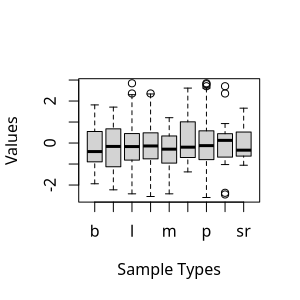
\includegraphics{images/ex1_box_300.png}
\textit{p: poblaci\'on, l: muestra de tama\~no 200, b: tama\~no 60, m: tama\~no 30 y s: tama\~no 20}.
\textit{Si tiene r al final es muestra con remplazo}

Para comparar los resultados utilizamos un gr\'afico de cajas y bisagras\footnote{No es posible aprecirlo bien en tama\~no tan reducido.}.
Los gr\'aficos de las muestras de tama\~no 200 se encuentran generalmente alineadas y bien formadas, indicador de que sus datos mantienen la distribuci�n normal de la poblaci\'on de la cual fueron extra\'idos.
La representaci\'on de cajas y bisagras de las otras muestras puede estar bien formada o no.
En la imagen ejemplo es posible ver que las muestras peque\~na sus datos no son representativos de la poblaci\'on,
al igual que la muestra de tama�o 60 sin remplazo, mientras que la muestra de tama\~no 60 con remplazo sus datos son representativos de la poblacion.

\subsection*{Intervalos de Confianza y diferencias entre las muestras de igual tama\~no}
Se estiman los intervalos de confianza para la media y la varianza con un nivle de signifacion del 5 por ciento. Luego se comparan los resultados entre las muestras de mismo tama�o.

Durante todas las pruebas realizadas todos los intervalos de confianza fueron correctos, es decir, la media y la varianza de la poblac\'ion siempre estuvieron dentro de los intervalos calculados.
No hubo una diferencia notable entre las muestras extraidas con remplazo y sin remplazo en sus intervalos de confianza.

\section*{Ejercicio 2} 

\section*{Ejercicio 3}
El problema trata sobre comparar la medias de a�os de educacion de los grupos de ingresos $\le50K$ y $>50K$, y ver si hay alguna diferencia significativa entre esas medias.\\
\textit{El c\'odigo referente a este ejercicio esta en el archivo exercise\_3.R}\\
Para lograr lo anterior se dividi\'o todos los datos del archivo csv en dos grupos: un grupo tiene ingresos $\le 50K$ y otro grupo tiene ingresos de $>50K$.\\
Luego de realizar la divisi\'on se escogieron dos muestras sin reemplazo de tama\~no $N= 60$ cada una.\\
Por lo que el problema se reduce a una prueba de hip�tesis para la comparaci�n de las medias de dos poblaciones Normales.\\
Las hip\'otesis para la prueba que se escogieron fueron:
$$
	H_0: \mu_1 = \mu_2
$$
$$
	H_1: \mu_1 \ne \mu_2
$$
Donde $\mu_1$ es la media de a\~nos de educaci\'on de la poblaci\'on de personas que poseen ingresos por debajo de los $50K$(inclusivo) y $\mu_2$ es la media de a\~nos de educaci\'on de la poblaci\'on de personas que poseen ingresos por encima de los $50K$.\\
Se asumi\'o que no se conoc\'ian las varianzas de dichos grupos(o que era muy costoso calcularlas). Por lo que para hacer la prueba de hip\'otesis de la media se hace primero una prueba de hip\'otesis para la igualdad de las varianzas.

\begin{lstlisting}[language=R,title=Parte del codigo para la hipotesis de varianza]
result <- var.test(sample1,
sample2, alternative = "two.sided")
\end{lstlisting}

Luego de establecer la igualdad o desigualdad de varianza se procede a realizar la prueba de la media:

\begin{lstlisting}[language=R,title=Parte del codigo para la hipotesis de la media]
result <-t.test(sample1,sample2, 
alternative = alt, var.equal = varequal)
\end{lstlisting}

Finalmente se compara el resultado del \textit{p-value} de \textit{result} con un valor $\alpha$ preestablecido y si es menor se rechaza la hip\'otesis nula.

\subsection*{Anal\'iticamente}
Se hace primero la prueba de varianza.\\
Los datos se tomaron del script referente al ejercicio.\\
$H_0: \sigma_1^2 = \sigma_2^2$\\
$H_1: \sigma_1^2 \ne \sigma_2^2$\\
$$
F = \frac{S_1^2}{S_2^2} = \frac{6.37}{5.13}= 1,24
$$
	$$
F_{1- \alpha /2}(n_1  - 1, n_2 - 1) = F_{0.975}(59,59) = 1.67
$$
$$
F_{\alpha/2}(n_1 -1, n_2-1) = F_{0.025}(59,59) =0.597
$$
Como $F> 	F_{\alpha/2}(n_1 -1, n_2-1)$ y $F< F_{1- \alpha /2}(n_1  - 1, n_2 - 1)$ no se puede descartar $H_0$ por lo que se asume que $\sigma_1^2 = \sigma_2^2$\\
$$
T_{\bar{X} - \bar{Y}} =	\frac{\bar{X} - \bar{Y}}{\sqrt{ (n_1 - 1)S_1^2 + (n_2 - 1)S_2^2   }}
\sqrt{\frac{n_1n_2(n_1+n_2-2)}{n_1 + n_2}} =3.7
$$
$$
t_{1-\alpha/2}(n_1+ n_2 -2) = t_{0.975}(116) =1.98
$$
Como $|T_{\bar{X} - \bar{Y}}| > t_{1-\alpha/2}(n_1+ n_2 -2)$ se cumple la regi\'on cr\'itica y se descarta $H_0$ pudiendo afirmarse que se aprecian diferencias significativas.



\section*{Conclusiones}

 (Cierta cantidad de minutos')
 
Se resumir\'an los resultados m\'as destacados ejercitados en la actividad.

Se puede hacer menci\'on de aplicaciones del m\'etodo estudiado, posibles investigaciones o repercusiones en la cotidianidad. As\'i como los elementos de mayor significaci\'on. 



\section*{Estudio Independiente}

(Algun tiempo')

Orientar y comentar los ejercicios siguientes:

\begin{eje}
	De creerlo conveniente, la asignaci\'on de tareas para el estudio independiente, o la asignaci\'on de evaluaciones. 
\end{eje}
\begin{eje}
	 La cantidad de los mismos es a conveniencia aunque podr\'ia ser de ayuda su justificaci\'on.
\end{eje}

\section*{Ejercicio 3}

Para concluir, la soluci\'on de los ejercicios propuestos.



\section*{Ejercicio 4}
El esquema de clase es variable y queda sujeto a la voluntad del participante, lo que si deber\'a ajustarse a los requisitos de la convocatoria oficial.


  
\end{document}
